This section presents three optimizations for structural bottlenecks and 
porting practices. Unless noted
otherwise, all performance measurements correspond to the 604M-cell
production case on 16 NVIDIA A100 GPUs (Section~\ref{sec:setup}).

\subsection{Chunk Pipelining across Serial Rank Chains}
\label{sec:opt-tridag}

\begin{figure}[h]
\centering
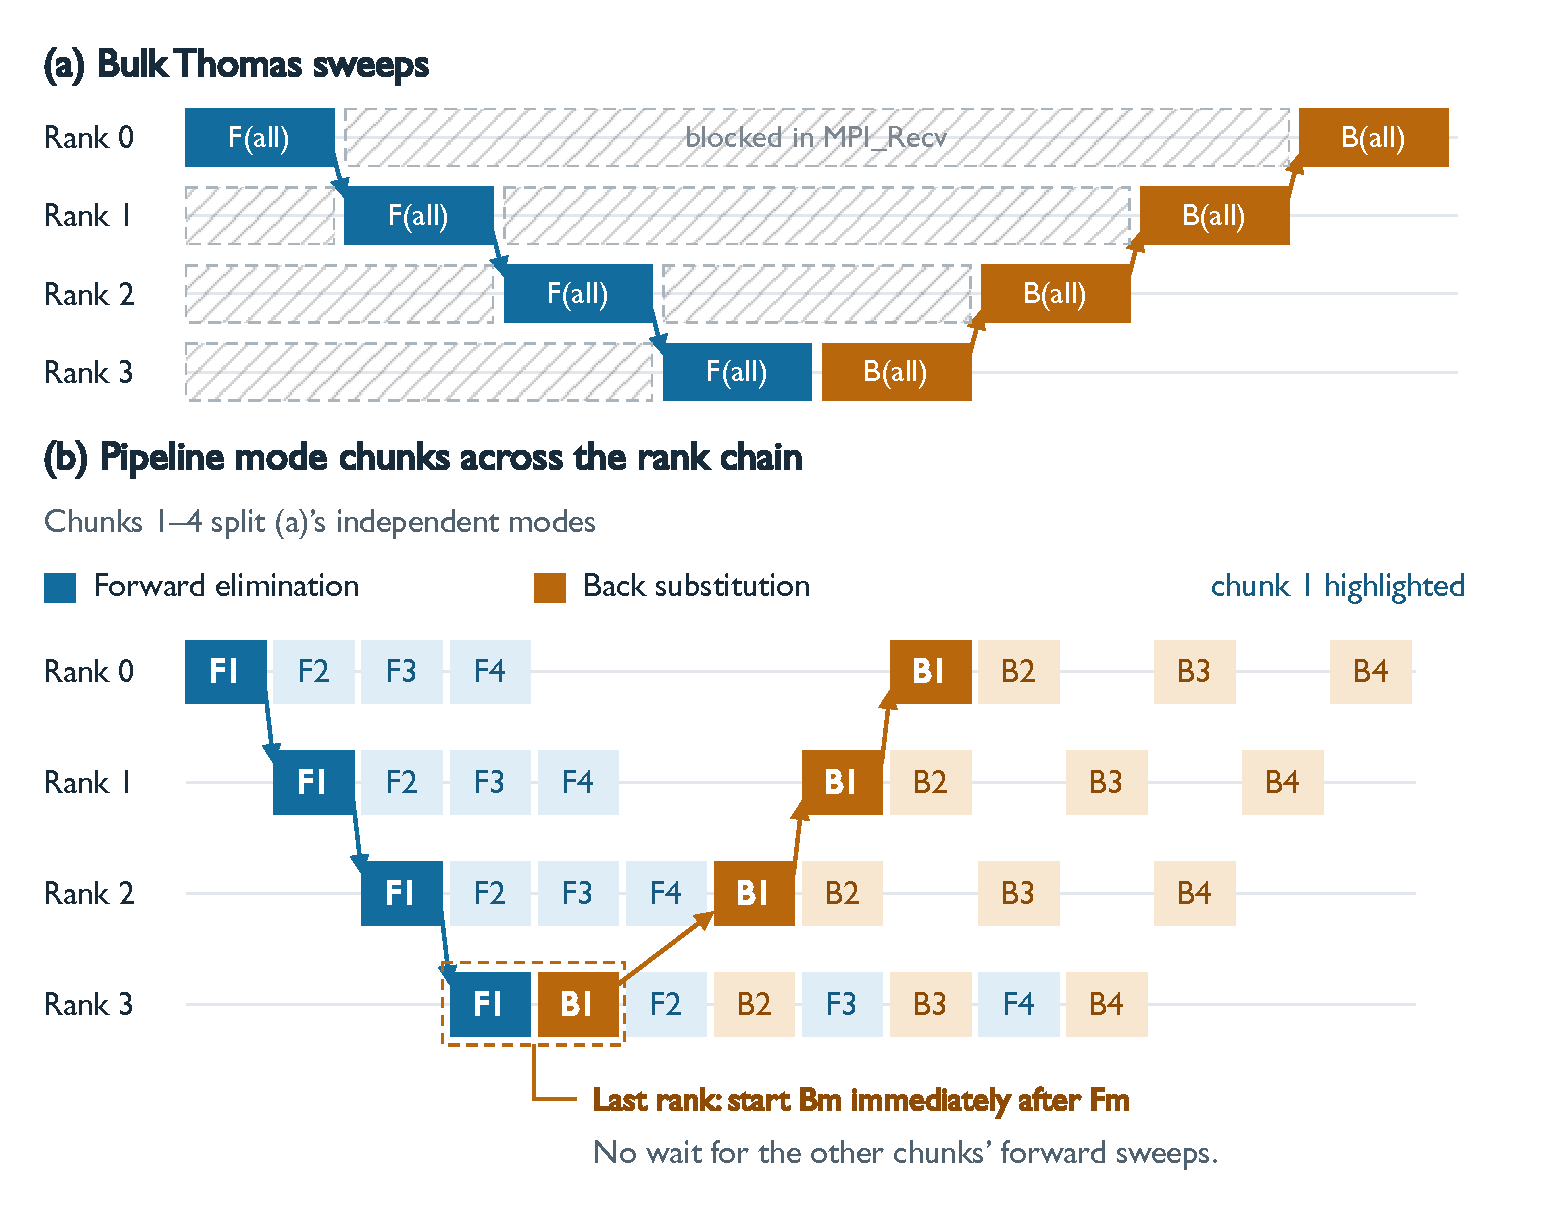
\includegraphics[width=\linewidth]{figs/fig4_lesgo_pipeline.pdf}
\caption{Pipelining the distributed Thomas solve. (a)~Sequential execution leaves ranks idle. (b)~Chunking overlaps forward elimination (blue) with boundary transfers and back substitution (orange).}
\label{fig:tridag}
\end{figure}

In the spectral Poisson solve (\texttt{PoissonTridiag()} in
Algorithm~\ref{alg:step}), independent 1D tridiagonal systems along $z$
arise for each horizontal wavenumber pair. This yields approximately
$590K$ independent systems of 512 unknowns, each distributed across
all 16 ranks in 1D slab domain decomposition. Standard forward
elimination and back substitution in the Thomas algorithm operate
serially along $z$, forcing rank $k$ to idle until rank $k-1$ completes
its forward pass.

To overcome this serialization, we exploit the mutual independence of these systems by partitioning them into $c$ chunks and pipelining the solve~\cite{povitsky1999,povitsky2000} (Fig.~\ref{fig:tridag}). In forward pass, rank $k$ processes chunk $m$, transmits boundary coefficients downstream to rank $k{+}1$, and immediately proceeds to chunk $m{+}1$.
Furthermore, chunking eliminates the global turnaround delay between forward elimination and back substitution. Ordinarily, back substitution must wait for the forward sweep to traverse the entire rank chain. Here, the last rank initiates back substitution for chunk $m$ as soon as its forward pass finishes, overlapping the backward wave of early chunks with the forward sweep of later ones. Unlike
reduced-system libraries that alter the elimination
arithmetic~\cite{laszlo2016,kim2021pascal}, our pipelined approach
leaves the inner Thomas loops untouched, ensuring results equivalence
with the sequential baseline.

\subsection{Batching Many Small Work Items}
\label{sec:opt-batch}

Several solver components decompose into many small, independent work
units. However, each unit is too lightweight to saturate the GPU on its own, 
and has fixed launching overhead. We batch these
units into fewer, larger device operations to amortize that overhead and
improve hardware occupancy.
We demonstrate this strategy with the actuator-line turbine model and the LASD subgrid-scale closure.

For the actuator-line model (\texttt{Turbines()}), 
processing turbines individually repeats device uploads, kernel
launches, synchronizations, and small collective reductions for each
turbine, accumulating over 1,000 \texttt{MPI\_Allreduce} operations per
rank every step. We therefore batch the entire farm into unified device
operations. Blade-point tables for all turbines reside permanently in
device memory. We use a single sampling kernel and a single projection kernel
process all concatenated turbine points, and all reduction quantities
travel in one packed \texttt{MPI\_Allreduce}. Together, these changes
cut per-step kernel launch and collective call counts by an order of
magnitude. The same restructuring also removed repeated device
allocations from the time loop, which
accelerated all other GPU solver stages by 15--18\%.

The Lagrangian scale-dependent (LASD) subgrid-scale model
(\texttt{UpdateLASDCoefficient()} in Algorithm~\ref{alg:step}) demonstrates the
same fragmentation. Each update filters nine 3D tensor fields at two 
test-filter scales: for every horizontal plane, it applies forward 2D FFTs, 
damps selected wavenumber modes, and applies inverse 2D FFTs. 
It also interpolates four accumulator fields to their upstream departure points
$x - u\,\Delta t$. A naive GPU port therefore issues thousands of
single-plane 2D FFTs per update, none large enough to saturate the
device. We therefore batch transforms along the
vertical dimension by promoting 2D scratch planes to 3D arrays, so that
a single batched cuFFT call filters all vertical levels of a field at
once. This consolidation collapses thousands of launches into a few dozen
while exposing enough parallel work per call to fully occupy the device.

\subsection{Heterogeneous CPU--GPU Execution}
\label{sec:opt-overlap}

\begin{figure}[h]
\centering
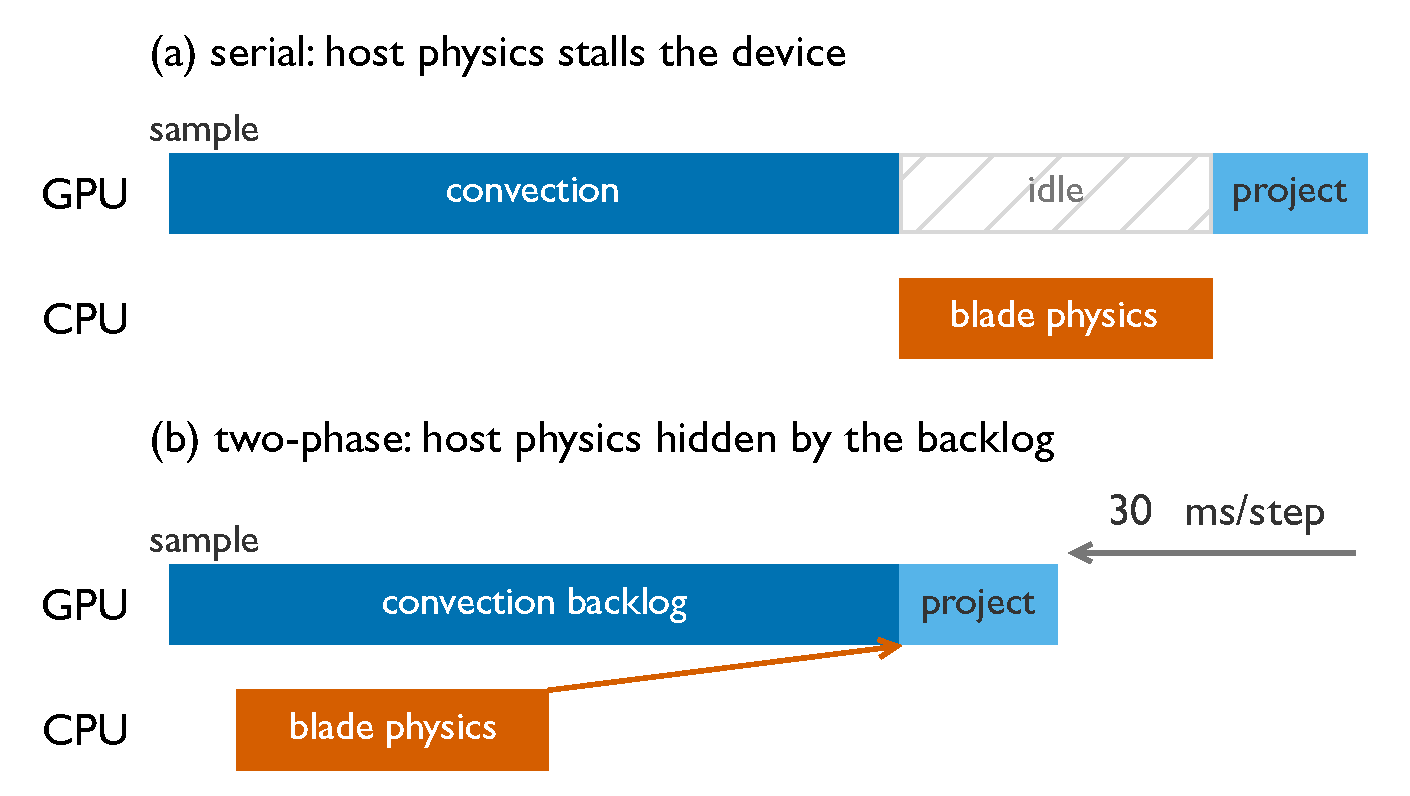
\includegraphics[width=\linewidth]{figs/fig_overlap.pdf}
\caption{Heterogeneous overlap of the actuator-line model.}
\label{fig:overlap}
\end{figure}

We initially ported every computational stage to the GPU, but found that
blade-force evaluation in the actuator-line model
(\texttt{ComputeBladeForces()} in Algorithm~\ref{alg:step}) actually ran
\emph{slower} on the device. 
The production case involves only 10,800 actuator points, far too few
to saturate a GPU. Moreover, each point traverses a data-dependent path
through the airfoil polar lookup, causing warps to serialize.
Kernel-launch and data-transfer overheads therefore exceed the useful
computation. We accordingly keep this routine. 
This decision, however, introduces a new challenge. Host execution
costs $\sim$28\,ms per step, and running it synchronously would leave
the GPU idle at every time step.
We address this by overlapping host computation with concurrent device
work.

Such overlap is feasible because blade-force evaluation only reads
velocities produced at the start of the time step, and its outputs are
not consumed until the force-projection stage later in the step. We
exploit this slack by splitting the actuator-line model into two
decoupled phases around the convection stage
(Fig.~\ref{fig:overlap}). Phase~1 samples blade-point velocities on the
GPU and transfers the compact data packet to the host, returning control
immediately without flushing the device queue. The GPU then proceeds
with convection while the CPU evaluates aerodynamic forces concurrently.
Phase~2 uploads the calculated forces and projects them onto the
Eulerian grid. 
This overlap removes host computation from the critical path, saving
30\,ms per step and raising overall GPU utilization to
\textbf{93\%}. This pattern generalizes to any host routine whose inputs
remain fixed at a known stage of the time step, effectively turning the
CPU into a coprocessor for code that resists GPU offloading.

\subsection{Experiences Porting to Modern GPUs}
\label{sec:opt-impl}

Beyond the optimizations above, we identified three general practices from
our porting effort that apply broadly to directive-based GPU codes.

\vspace{0.08in}
\textbf{Compute Uniformly, Then Patch the Exceptions.} Conditional
logic inside a hot kernel forces every thread in a warp to serialize
along divergent paths, even threads that never take the branch. When
the exceptional points form a lower-dimensional subset of the iteration
space, such as $O(N^2)$ boundary cells versus $O(N^3)$ interior cells,
this penalty is easy to avoid. We use the uniform interior stencil
over the entire domain in a single branch-free kernel with coalesced
accesses, then overwrite boundary values with a second, far smaller
patch kernel. The redundant work is negligible compared to the volume
computation.

\vspace{0.08in}
\textbf{Derive the Parallel Domain from the Data, Not the Loop Nest.}
Translating CPU loop nests directly into GPU kernels tends to inherit
the serial structure of the original code, with poor occupancy and
strided memory traffic. We instead let the data layout
drive the thread decomposition. For regular stencil kernels, we
collapse all spatial loops with the contiguous index innermost so that
warps issue coalesced loads. For work scattered across many small model
instances, we flatten all instances into a single parallel domain of
work items, one thread per item regardless of which instance owns it.

\vspace{0.08in}
\textbf{Align Code Structure with Compiler Offloading Models.} The
NVHPC compiler places small local-array temporaries in thread-private
local memory, which is backed by device DRAM and far slower than
registers. We scalar expand these temporaries so that the compiler can
promote them to registers. 
% We treat the diagnostic output from \texttt{-Minfo=accel} as a mandatory 
% build check to verify that it does so. 
Besides, we found that OpenACC allocates per-thread temporary arrays for every
invocation of Fortran array-valued functions and utility routines. This
means each such call generates device DRAM traffic with substantial
overhead. We therefore manually inline these routines at their call
sites to eliminate the allocation entirely. 